\documentclass [11pt]{book}

\author {Dave Cooper}

\textwidth 6.5in

\topmargin 0in

\textheight 8.5in

\oddsidemargin 0in

\evensidemargin 0in

\pdfimageresolution 135

\title {GenDL Unified Documentation}

\usepackage [dvips]{graphicx}

\usepackage [usenames, dvipsnames]{color}

\usepackage {makeidx}

\usepackage {textcomp}

\usepackage [colorlinks=true, urlcolor=cyan]{hyperref}

\newsavebox {\boxedverb}

\makeindex 



\begin{document}



\frontmatter



\maketitle


\footnotetext{Copyright 
\copyright{} 2012, Genworks International. Duplication, by any means, in whole or in part, requires 
written consent from Genworks International.}

\tableofcontents



\mainmatter



\chapter{Introduction}

\label{chap:introduction}



\section{Welcome}

\label{sec:welcome}

Congratulations on your purchase or download of Genworks Gendl. By investing some of your 
valuable time into learning this system, you are investing in your future productivity and you are becoming
part of a quiet revolution. Although you may have come to Genworks Gendl because of an interest in 3D modeling
or mechanical engineering, you will find that a whole new world, and a whole new approach to computing, will 
now be at your fingertips.

\section{Knowledge Base Concepts According to Genworks}

\label{sec:knowledgebaseconceptsaccordingtogenworks}

You may have an idea about Knowledge Base Systems,
or Knowledge \emph{Based} Systems, from college textbooks or corporate marketing propaganda, and found the 
concept too broad to be of practical use. Or you may have heard jabs at the 
pretentious-sounding name, ``Knowledge-based Engineering,'' as in: ``you mean as opposed to \index{Ignorance-based Engineering}Ignorance-based Engineering?'' 

To provide a clearer picture, we hope you will agree that our concept
of a KB system is simple and practical, and in this tutorial our goal
is to make you comfortable and excited about the ideas we have
implemented in our flagship system, GenDL (or ``Gendl'' 


Our definition of a \emph{\index{Knowledge Base System}Knowledge Base System} is an object-oriented programming environment which implements the features of \emph{\index{Caching}Caching} and \emph{\index{Dependency tracking}Dependency tracking}. Caching means that once the KB has computed something, it might not need to repeat 
that computation if the same question is asked again. Dependency tracking is the flip side
of that coin --- it ensures that if a cached result is \emph{stale}, the result will be recomputed the next time it is \emph{demanded}, so as to give a fresh result.

\section{Goals for this Tutorial}

\label{sec:goalsforthistutorial}

This manual is designed as a companion to a live two-hour GDL/GWL tutorial, but you may
also be reading it on your own. In either case, the basic goals are:

\begin{itemize}

\item Get you excited about using GDL/GWL

\item Enable you to judge whether GDL/GWL is an appropriate tool for a given job

\item Arm you with the ability to argue the case for using GDL/GWL when appropriate

\item Prepare you to begin maintaining and authoring GDL/GWL applications, or porting apps
from similar KB systems into GDL/GWL.

\end{itemize}

This manual will begin with an introduction to the \index{Common Lisp}Common Lisp programming language. If you are new to Common Lisp:
congratulations! You have just discovered a powerful tool backed by a
powerful standard specification, which will protect your development
investment for decades to come. In addition to the brief overview in
this manual, many resources are available to get you started in CL ---
for starters, we recommend 
\underline{\index{Basic Lisp Techniques}Basic Lisp Techniques}\footnote{
\underline{BLT} is available at \texttt{http://www.franz.com/resources/educational\_resources/cooper.book.pdf}}, which was prepared by the author of this tutorial. 

\section{What is GenDL?}

\label{sec:whatisgendl?}

GenDL (or Gendl to be a bit more relaxed) is an acronym for
``General-purpose Declarative Language.'' 

GenDL is a superset of ANSI Common Lisp, and consists mainly of
automatic code-expanding extensions to Common Lisp implemented in the
form of macros. When you write, let's say, 20 lines in GenDL, you
might be writing the equivalent of 200 lines of Common Lisp. Of
course, since GenDL is a superset of Common Lisp, you still have the
full power of the CL language at your fingertips whenever you are
working in GenDL.

\index{compiled language!benefits of}\index{macros!code-expanding}Since GDL expands into CL, everything you write in GDL will be
compiled ``down to the metal'' to machine code with all the
optimizations and safety that the tested-and-true CL compiler
provides. This is an important distinction as contrasted to some other
so-called KB systems on the market, which are really nothing more than
interpreted scripting languages which often impose arbitrary limits on
the size and complexity of your application.

GenDL is also a true \emph{\index{declarative}declarative} language. When you put together a GDL application, you write and think mainly
in terms of objects and their properties, and how they depend on one another in a direct
sense. You do not have to track in your mind explicitly how one object or property will ``call''
another object or propery, in what order this will happen, etc. Those details are
taken care of for you automatically by the language. 

Because GDL is object-oriented, you have all the features you would normally expect
from an object-oriented language, such as 

\begin{itemize}

\item Separation between the \emph{definition} of an object and an \emph{instance} of an object

\item High levels of data abstraction

\item The ability for one object to ``inherit'' from others

\item The ability to ``use'' an object without concern for its ``under-the-hood'' implementation

\end{itemize}

\index{object-orientation!message-passing}\index{object-orientation!generic-function}GDL supports the ``message-passing'' paradigm of object orientation, with some extensions. Since
full-blown ANSI CLOS (Common Lisp Object System) is always available as well, the Generic Function paradigm 
is supported as well. Do not be concerned at this point if you are not fully aware of the differences 
between these two paradigms\footnote{See Paul Graham's 
\underline{ANSI Common Lisp}, page 192, for an excellent discussion of the Two Models 
of Object-oriented Programming.}.

\section{Why GDL (what is GDL good for?)}

\label{sec:whygdl(whatisgdlgoodfor?)}



\begin{itemize}

\item Organizing and interrelating large amounts of information
in ways not possible or not practical using conventional languages or 
conventional relational database technology alone;

\item Evaluating many design or engineering alternatives and 
performing various kinds of optimizations within specified design
spaces;

\item Capturing the procedures and rules used to solve repetitive
tasks in engineering and other fields;

\item Applying rules to achieve intermediate and final 
outputs, which may include virtual models of wireframe, surface,
and solid geometric objects.

\end{itemize}



\section{What GDL is not}

\label{sec:whatgdlisnot}



\begin{itemize}

\item A CAD system (although it may operate on and/or generate geometric entities);

\item A drawing program (although it may operate on and/or generate geometric entities);

\item An Artificial Intelligence system (although it is an excellent environment for developing 
capabilities which could be considered as such);

\item An Expert System Shell (although one could be easily embedded within it).

\end{itemize}

Without further ado, then, let's turn the page and get started with some hands-on GDL...

\chapter{Installation}

\label{chap:installation}

Follow Section 
\ref{sec:installationofpre-packagedgendl} if your email address is registered with Genworks and you will
install a pre-packaged Gendl distribution including its own Common
Lisp engine.  Gendl is also available as open-source software\footnote{http://github.com/genworks/Genworks-GDL}; if you
want to use that version, then please refer to Section 
\ref{sec:installationofopen-sourcegendl}.

\section{Installation of pre-packaged Gendl}

\label{sec:installationofpre-packagedgendl}

This section will take you through the installation of Gendl
from a prepackaged distribution with the Allegro CL Common Lisp engine
and the Slime IDE (based on Gnu Emacs).

\subsection{Download the Software and retrieve a license key}

\label{subsec:downloadthesoftwareandretrievealicensekey}



\begin{enumerate}

\item Visit the Downloads section of the \href{http://genworks.com/newsite}{Genworks Newsite}

\item Enter your email address\footnote{if your address is not on file, send mail to licensing@genworks.com}.

\item Download the latest Payload and gpl.zip for Windows\footnote{If you already have a gpl.zip from a previous Gendl installation, it is not necessary to download a new one.}

\item Click to receive license key file by email.

\end{enumerate}



\subsection{Unpack the Distribution}

\label{subsec:unpackthedistribution}

GenDL is currently distributed for all the platforms as a
self-contained ``zip'' file which does not require official
administrator installation.  What follows are general instructions; more up-to-date details
may be found in the email which accompanies the license key file. A five-minute installation video
is also available in the Documentation section of the \href{http://genworks.com/newsite}{Genworks Newsite}.

\begin{enumerate}

\item Unzip the gdl1581... zipfile into a location where you have write permissions

\item Unzip the gpl.zip file at the same level as the gdl payload

\item Copy the license key file as gdl.lic (for Trial,
	 Student, Professional editions), or devel.lic (for Enterprise edition) into the \texttt{program/} directory within the gdl1581.../ directory.

\end{enumerate}


\begin{figure}
\begin{center}
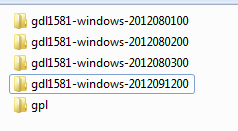
\includegraphics{../images/gendl-installation.png}
\end{center}

\caption{Several Gendl versions and one GPL }

\label{fig:gendl-installation}

\end{figure}
So you now should have two directories at the same level: one named \texttt{gdl1581.../}(the rest of the name will contain the specific dated build stamp), and a \texttt{gdl/}directory at the same level. Note that as seen in Figure 
\ref{fig:gendl-installation}, it is possible to have several Gendl versions installed, but just a single common \texttt{gpl/} folder.

\subsection{Make a Desktop Shortcut}

\label{subsec:makeadesktopshortcut}



\begin{enumerate}

\item Using the ``My Computer'' or ``Computer'' Windows file manager, right-mouse on the \texttt{run-gdl.bat} file.

\item Select ``Create Shortcut.''

\item Now drag the new ``Run-gdl-shortcut'' icon to your desktop.

\end{enumerate}



\subsection{Populate your Initialization File}

\label{subsec:populateyourinitializationfile}

The default initialization file for Gendl is called \texttt{gdlinit.cl}, 

\section{Installation of open-source Gendl}

\label{sec:installationofopen-sourcegendl}

This section is only relevant if you have not received a
pre-packaged Gendl distribution with its own Common Lisp engine.  If
you have received a pre-packaged Gendl distribution, then please skip
this section. In case you want to use the open-source Gendl, you will
use your own Common Lisp installation and fetch Gendl (Genworks-GDL)
using a very powerful and convenient CL package/library manager
called \emph{Quicklisp}.

\subsection{Install and Configure your Common Lisp environment}

\label{subsec:installandconfigureyourcommonlispenvironment}

Gendl is currently tested to build on the following Common Lisp engines:

\begin{itemize}

\item Allegro CL (commercial product from Franz Inc, free Express Edition available)

\item LispWorks (commercial product from LispWorks Ltd, free Personal Edition available)

\item Steel Bank Common Lisp (SBCL) (free open-source project with permissive license)

\end{itemize}

Please refer to the documentation for each of these systems for full information on installing 
and configuring the environment. Typically this will include a text editor, either Gnu Emacs with Superior
Lisp Interaction Mode for Emacs (Slime), or a built-in text editing and development environment which 
comes with the Common Lisp system.

As of this writing, a convenient way to set up Emacs with Slime is to use the \href{http://github.com/quicklisp/quicklisp-slime-helper}{Quicklisp-slime-helper}.

\subsection{Load and Configure Quicklisp}

\label{subsec:loadandconfigurequicklisp}

As of this writing, Quicklisp is rapidly becoming the defacto standard library manager for Common Lisp.

\begin{itemize}

\item Visit the \href{http://quicklisp.org}{Quicklisp website}

\item Follow the instructions there to download the \texttt{quicklisp.lisp} bootstrap file and load it to set up your Quicklisp environment.

\end{itemize}



\section{System Startup and Testing}

\label{sec:systemstartupandtesting}



\subsection{System Startup}

\label{subsec:systemstartup}



\subsubsection{Startup of prepackaged Gendl distribution}

\label{subsubsec:startupofprepackagedgendldistribution}

To start a prepackaged system, follow these steps:

\begin{enumerate}

\item Invoke the \texttt{run-gdl.bat} (Windows), or \texttt{run-gdl} (Linux, MacOS) startup script. This should launch Gnu Emacs with a 
README file displayed by default. Take the time to look through this README file. 
Especially the later part of the file contains information about Emacs keyboard
shortcuts available.

\item In emacs, enter: \texttt{M-x glime}. That is, hold down the ``Meta'' (or ``Alt'') key, and press the ``X'' key, then type ``glime.''
You will see this command shown in the \emph{mini-buffer} at the bottom of the Emacs window, as shown in Figure 
\ref{fig:mini-buffer}

\begin{figure}
\begin{center}
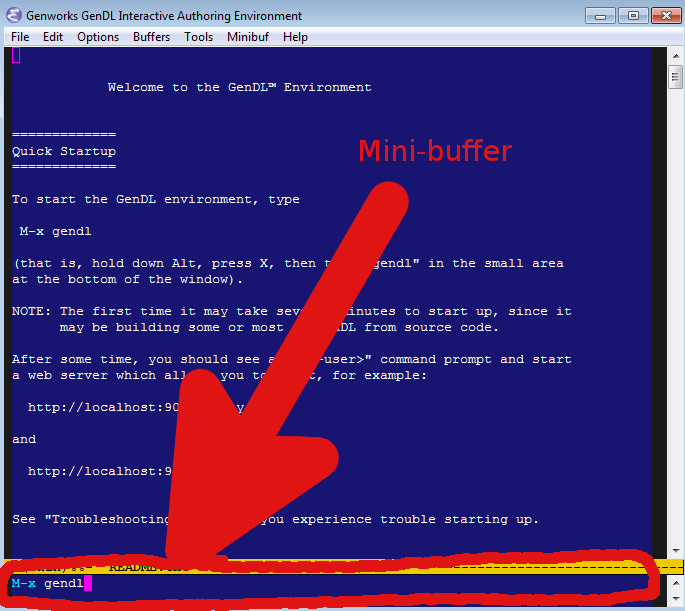
\includegraphics[width=3in,height=3in]{../images/mini-buffer.png}
\end{center}

\caption{The mini-buffer in Emacs}

\label{fig:mini-buffer}

\end{figure}

\item press the ``Enter'' key

\begin{figure}
\begin{center}
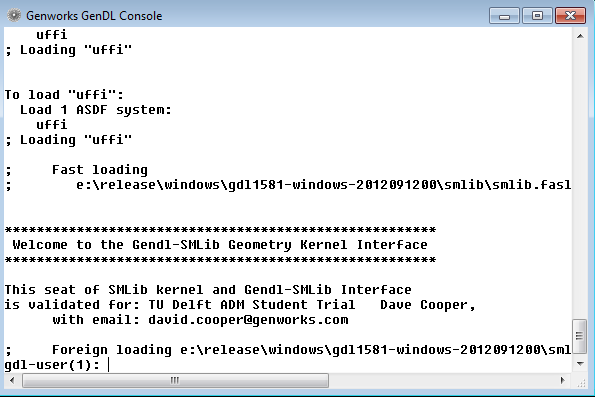
\includegraphics{../images/genworks-gendl-console.png}
\end{center}

\caption{Genworks Gendl Console}

\label{fig:genworks-gendl-console}

\end{figure}

\item On Windows, you will get a new window, named the the \index{Genworks Gendl Console}Genworks Gendl Console, as shown in Figure 
\ref{fig:genworks-gendl-console}. This window might start out in minimized form (as an icon at the bottom of your screen). Click on it 
to open it. Watch this console for any errors or warnings. 

The first time you start up, you may see messages in this console for
several minutes while the system is being built (or if you received a
completely pre-built system, the messages may last only a few
seconds).

On Linux or MacOS, there will be a separate Emacs buffer (available
through Emacs' ``Buffers'' menu) where you will see these messages.

The messages will consist of compiling and loading information, followed by copyright and welcome information
for Gendl. After these messages have finished, you should see the following command prompt:

\texttt{\index{gdl-user(1): }gdl-user(1): }

The Genworks GenDL console contains a command prompt, but mostly you will use the \index{*slime-repl...*}*slime-repl...* buffer in Emacs to type commands. The Genworks GenDL console is mainly used for 
displaying output text from the Gendl system and from your application.

\end{enumerate}



\subsubsection{Startup of open-source Gendl distribution}

\label{subsubsec:startupofopen-sourcegendldistribution}

To start an Open-source distribution, follow these steps:

\begin{enumerate}

\item Start your Common Lisp engine and development environment (e.g. SBCL with Emacs and Superior Lisp Interaction Mode for Emacs).

\item After Quicklisp is installed and initialized in your system, type: \texttt{(ql:quickload :genworks-gdl)} to get Genworks Gendl installed and loaded in your environment.

\item Type the following to initialize the Gendl environment:

\texttt{(gdl:start-gdl :edition :open-source)}



\end{enumerate}



\subsection{Basic System Test}

\label{subsec:basicsystemtest}

You may test your installation using the following
checklist. These tests are optional. You may perform some or all of
them in order to ensure that your Gendl is installed correctly and
running smoothly. In your Web Browser (e.g. Google Chrome, Firefox,
Safari, Opera, Internet Explorer), perform the following steps:

\begin{enumerate}

\item visit http://localhost:9000/tasty.

\item accept default robot:assembly.

\item Select ``Add Leaves'' from the Tree menu.

\item Click on the top node in the tree.

\item Observe the wireframe graphics for the robot as shown in 
\ref{fig:tasty-robot}.

\begin{figure}
\begin{center}
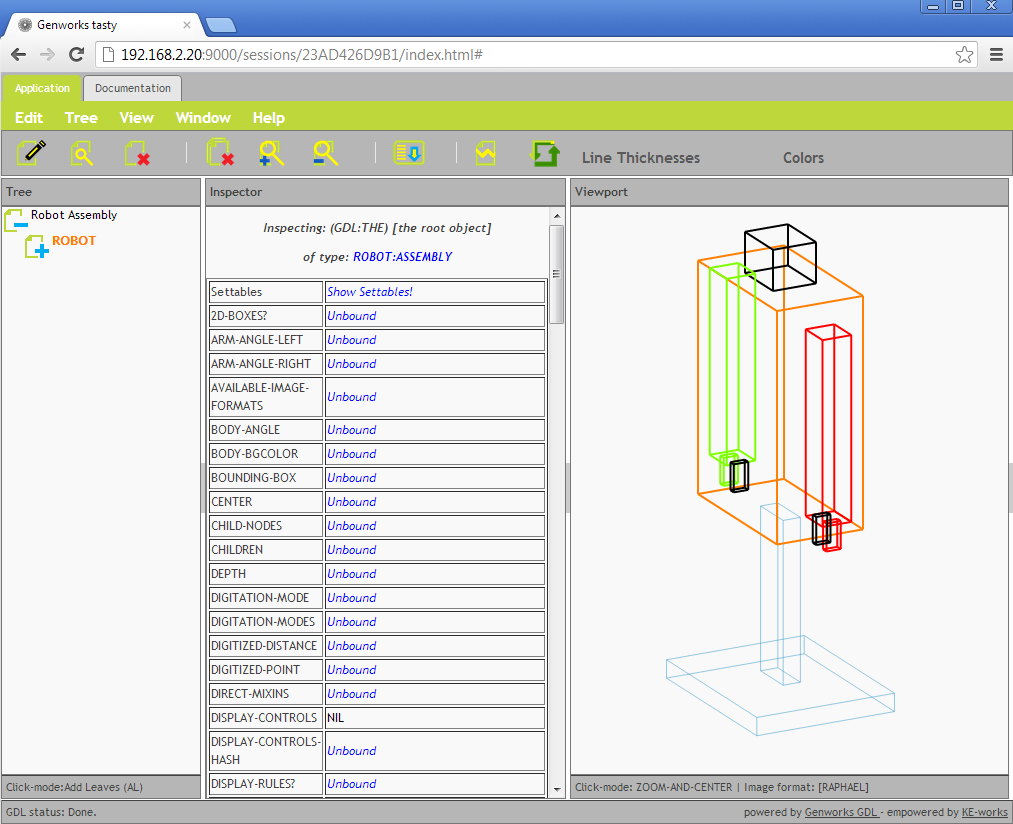
\includegraphics[width=3in,height=3in]{../images/tasty-robot.png}
\end{center}

\caption{Robot displayed in Tasty}

\label{fig:tasty-robot}

\end{figure}

\begin{figure}
\begin{center}
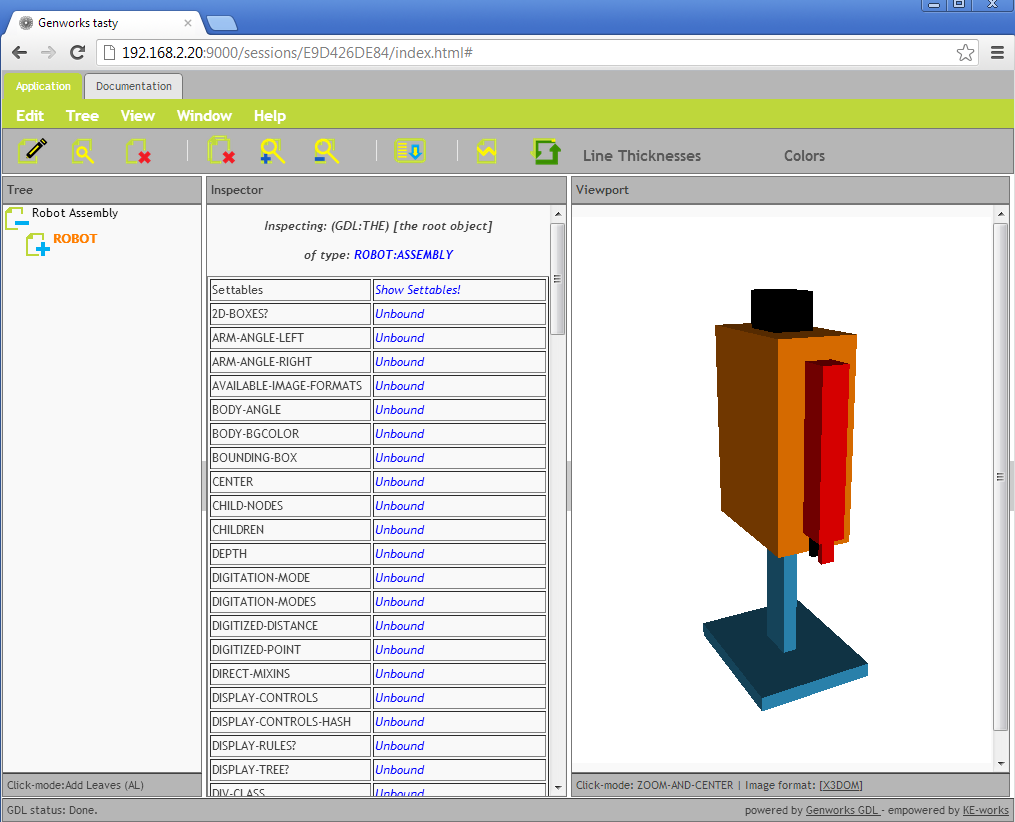
\includegraphics[width=3in,height=3in]{../images/tasty-robot-x3dom.png}
\end{center}

\caption{Robot x3dom}

\label{fig:tasty-robot-x3dom}

\end{figure}

\item Click on the robot to zoom in.

\item Select ``Clear View!'' from the View menu.

\item Select ``X3DOM'' from the View menu.

\item Click on the top node in the tree.

\item ``Refresh'' or ``Reload'' your browser window (may not be necessary).

\item If your browser supports WebGL, you will see the robot in shaded dynamic view as shown in Figure
\ref{fig:tasty-robot-x3dom}.

\item Select ``PNG'' from the View menu. You will see the wireframe view of the robot as a PNG image.

\item Select ``X3D'' from the View menu. If your browser has an X3D plugin installed (e.g. BS Contact), 
you will see the robot in a shaded dynamic view.

\end{enumerate}



\subsection{Full Regression Test}

\label{subsec:fullregressiontest}

\index{regression tests}The following commands will invoke a full regression test, including a test of the Surface and Solids
primitives provided by the SMLib geometry kernel. Note that the SMLib geometry kernel is only available with
proprietary Gendl licenses --- therefore if you have an open-source or Trial version, you these regression
tests will not all function.

In Emacs at the \texttt{gdl-user>} prompt in the \texttt{*slime-repl...*} buffer, type the following commands:

\begin{enumerate}

\item \texttt{(ql:quickload :gdl-regression)}

\item \texttt{(gdl-lift-utils::define-regression-tests)}

\item \texttt{(gdl-lift-utils::run-regression-tests-pass-fail)}

\item \texttt{(pprint gdl-lift-utils::*regression-test-report*)}

\end{enumerate}



\section{Getting Help and Support}

\label{sec:gettinghelpandsupport}

If you run into unexplained errors in the installation and startup process, please contact the following resources:

\begin{enumerate}

\item Make a posting to the \href{http://groups.google.com/group/genworks}{Genworks Google Group}

\item For pure Common Lisp issues, join the \#lisp IRC (Internet Relay Chat) channel and discuss issues there.

\item Also for Common Lisp issues, follow the comp.lang.lisp Usenet group.

\item If you are a supported Genworks customer, send email to \href{mailto:support@genworks.com}{support@genworks.com}

\item If you are not a supported Genworks customer but you want to report an apparent bug or have other suggestions or inquiries, you may also send email to \href{mailto:support@genworks.com}{support@genworks.com}, but please understand that Genworks cannot guarantee any response or a particular timeframe for any response.

\end{enumerate}



\chapter{Basic Operation of the Gendl Environment}

\label{chap:basicoperationofthegendlenvironment}

This chapter will step you through all the basic steps of
operating a typical Gendl environment. We will not go into any depth
about the additional features of the environment or language syntax in
this section --- this is just for getting familiar and practicing with
the mechanics of operating the environment with a keyboard.

\section{What is Different about Gendl?}

\label{sec:whatisdifferentaboutgendl?}

Gendl is  a dynamic language environment with incremental compiling and in-memory 
definitions. That means that as long as the system is running, you can \emph{compile} new \emph{definitions} of functions, objects, etc, and they will immediately become available as part of the running system,
and you can begin testing them immediately or update an existing set of objects to observe their new behavior.

In many other programming language systems, you have to start the
system from the beginning and reload all the files in order to test
new functionality. 
 
In Gendl, if you simply shut down the system after having compiled and
loaded a set of files with new definitions, then when you restart the
system you will have to recompile and/or reload those definitions in
order to bring the system back into the same state. This is typically
done automatically, using commands placed into the \texttt{gdlinit.cl} initialization file, as introduced in Section 
\ref{sec:customizingyourenvironment}. Alternatively, you can compile and load definitions into your Gendl
session, then save the ``world'' in that state. That way, it is
possible to start a new Gendl ``world'' which already has all your
application's definitions loaded and ready for use, without having to
procedurally reload any files. You can then begin to make and test new
definitions (and re-definitions) starting from this new ``world.''

\section{Startup, ``Hello, World!'' and Shutdown}

\label{sec:startup,hello,world!andshutdown}



The typical Gendl environment consists of three programs: Gnu
Emacs (the editor), a Common Lisp engine with Gendl system loaded or built into it (e.g. the \texttt{gdl.exe} executable in your \texttt{program/} directory), and (optionally) a web browser
such as Firefox, Google Chrome, Safari, Opera, or Internet
Explorer. Emacs runs as the main \emph{process}, and this in turn starts the CL engine with Gendl as a \emph{sub-process}. The CL engine typically runs an embedded \emph{webserver}, enabling you to access your application through a standard web browser.



As introduced in Chapter 
\ref{chap:installation}, the typical way to start a pre-packaged Gendl environment is with the \texttt{run-gdl.bat} (Windows), or \texttt{run-gdl} (MacOS, Linux) script files. Invoke this script file
from your computer's file manager, or from a desktop shortcut if you
have created one as outlined in section 
\ref{subsec:makeadesktopshortcut}. Your installation executable may also have created a
Windows ``Start'' menu item for Genworks Gendl. Of course you can also 
invoke \texttt{run-gdl.bat} from the Windows ``cmd'' command-line, or from another command shell such as Cygwin.\footnote{Cygwin is also useful as a command-line tool on Windows
for interacting with a version control system like Subversion (svn).}



\subsection{Startup}

\label{subsec:startup}

 Startup of a typical Gendl development session consists of
two fundamental steps: (1) starting the Emacs editing environment,
and (2) starting the actual Gendl process as a ``sub-process'' or ``inferior'' process 
within Emacs. The Gendl process should automatically establish a network connection
back to Emacs, allowing you to interact directly with the Gendl process from within Emacs.

\begin{enumerate}

\item Invoke the \texttt{run-gdl.bat} or \texttt{run-gdl.bat} startup script.

\item You should see a blue emacs window as in Figure 
\ref{fig:emacs-startup}. (alternative colors are also possible).

\item Press M-x (Alt-x), and type \texttt{gendl} in the mini-buffer, as seen in Figure 
\ref{fig:mini-buffer}.

\item (MS Windows): Look for the Genworks Gendl Console
window, or (Linux, Mac) use the Emacs ``Buffer'' menu to visit the
``*inferior-lisp*'' buffer. Note that the Genworks Gendl Console
window might start as a minimized icon; click or double-click it to
un-minimize.

\item Watch the Genworks GDL Console window for any
errors. Depending on your specific installation, it may take from a
few seconds to several minutes for the Genworks Gendl Console (or
*inferior-lisp* buffer) to settle down and give you a \texttt{gdl-user(): } prompt. This window is where you will see most of your program's textual output, any 
error messages, warnings, etc.

\item In Emacs, type: \texttt{C-x \&} (or select Emacs menu item Buffers$\rightarrow$*slime-repl...*) to visit the ``*slime-repl ...*'' buffer. The full name
of this buffer depends on the specific CL/Gendl platform which you are
running. This buffer contains an interactive prompt, labeled \texttt{gdl-user>}, where you will enter most of your commands to interact with your running Gendl session
for testing, debugging, etc. There is also a web-based graphical interactive environment called \emph{tasty} which will will cover in Chapter 
\ref{chapter:tasty}

\item To ensure that the Gendl interpreter is up and running, type: \texttt{(+ 2 3)} and press [Enter].

\item You should see the result \texttt{5} echoed back to you below the prompt.

\end{enumerate}



\subsection{Developing and Testing a Gendl ``Hello World'' application}

\label{subsec:developingandtestingagendlhelloworldapplication}

 

\begin{enumerate}

\item type C-x (Control-x) 2, or C-x 3, or use the ``Split
Screen'' option of the File menu to split the Emacs frame into two
``windows'' (``windows'' in Emacs are non-overlapping panels, or
rectangular areas within the main Emacs window).

\item type C-x o several times to move from one window to
the other, or move the mouse cursor and click in each window. Notice
how the blinking insertion point moves from one window to the other.

\item In the top (or left) window, type C-x C-f (or select Emacs menu item
``File$\rightarrow$Open File'') to get the ``Find file'' prompt in the
mini-buffer.

\item Type C-a to move the point to the beginning of the mini-buffer line.

\item Type C-k to delete from the point to the end of the mini-buffer.

\item Type \texttt{\textasciitilde/hello.gdl} and press [Enter]

\item You are now editing a (presumably new) file of Gendl
	 code, located in your HOME directory, called \texttt{hello.gdl}

\item Enter the text from Figure 
\ref{fig:simpleobjectdefinition} into the \texttt{hello.gdl} buffer. You do not have to match the line breaks and whitespace as shown in the example.
You can auto-indent each new line by pressing [TAB] after pressing [Enter] for the newline.

\emph{Protip:}You can also try using \texttt{C-j} instead of [Enter], which will automatically give a newline and auto-indent.



\begin{figure}
\begin{lrbox}{\boxedverb}
\begin{minipage}{\linewidth}

\begin{verbatim}
 (in-package :gdl-user)

 (define-object hello ()

   :computed-slots 
   ((greeting "Hello, World!")))

\end{verbatim}
\end{minipage}
\end{lrbox}
\fbox{\usebox{\boxedverb}}

\caption{Example of Simple Object Definition}

\label{fig:simpleobjectdefinition}

\end{figure}

\item type \texttt{C-x C-s} (or choose Emacs menu item \emph{File$\rightarrow$Save}) to save the contents of the buffer (i.e. the window) 
to the file in your HOME directory.

\item type \texttt{C-c C-k} (or choose Emacs menu item \emph{SLIME$\rightarrow$Compilation$\rightarrow$Compile/Load File}) to compile \& load the code from this file.

\item type \texttt{C-c o} (or move and click the mouse)  to switch to the bottom window.

\item In the bottom window, type \texttt{C-x \&} (or choose Emacs menu item \emph{Buffers$\rightarrow$*slime-repl...*}) to get the \texttt{*slime-repl ...*} buffer, which should contain a \texttt{gdl-user>} prompt. This is where you normally type interactive Gendl commands.

\item If necessary, type \texttt{M \textgreater} (that is, hold down Meta (Alt), Shift, and the ``\textgreater'' key) to
move the insertion point to the end of this buffer.

\item At the \texttt{gdl-user>} prompt, type 

\begin{verbatim}(make-self 'hello)
\end{verbatim} and press [Enter].

\item At the \texttt{gdl-user>} prompt, type 

\begin{verbatim}(the greeting)
\end{verbatim} and press [Enter].

\item You should see the words \texttt{Hello, World!} echoed back to you below the prompt.

\end{enumerate}



\subsection{Shutdown}

\label{subsec:shutdown}

 To shut down a development session gracefully, you should first shut down the Gendl process,
then shut down your Emacs.

\begin{itemize}

\item Type \texttt{M-x quit-gendl} (that is, hold Alt and press X, then release both while you type \texttt{quit-gendl} in the mini-buffer), then press [Enter]

\item Type \texttt{C-x C-c} to quit from Emacs. Emacs will prompt you to save any modified buffers before exiting.

\end{itemize}



\section{Working with Projects}

\label{sec:workingwithprojects}

Gendl contains utilities which allow you to treat your
application as a ``project,'' with the ability to compile,
incrementally compile, and load a ``project'' from a directory tree of
source files representing your project. In this section we give an
overview of the expected directory structure and available control
files, followed by a reference for each of the functions included in
the bootstrap module.

\subsection{Directory Structure}

\label{subsec:directorystructure}



You should structure your applications in a modular fashion, with the
directories containing actual Lisp sources called "source."



You may have subdirectories which themselves contain "source"
directories.



We recommend keeping your codebase directories relatively flat,
however.



In Figure 
\ref{fig:yoyodyne-base} is an example application directory, with four source files.


\begin{figure}
\begin{lrbox}{\boxedverb}
\begin{minipage}{\linewidth}

\begin{verbatim}
  apps/yoyodyne/booster-rocket/source/assembly.gdl
  apps/yoyodyne/booster-rocket/source/package.gdl
  apps/yoyodyne/booster-rocket/source/parameters.gdl
  apps/yoyodyne/booster-rocket/source/rules.gdl

\end{verbatim}
\end{minipage}
\end{lrbox}
\fbox{\usebox{\boxedverb}}

\caption{Example project directory with four source files}

\label{fig:yoyodyne-base}

\end{figure}


\subsection{Source Files within a source/ subdirectory}

\label{subsec:sourcefileswithinasource/subdirectory}



\subsubsection{Enforcing Ordering}

\label{subsubsec:enforcingordering}



Within a source subdirectory, you may have a file called \texttt{file-ordering.isc}\footnote{\texttt{isc} stands for ``Intelligent Source Configuration''} to enforce a certain ordering on the files. Here is the contents of an example for the 
above application:



\texttt{("package" "parameters")}



This will force package.lisp to be compiled/loaded first, and
parameters.lisp to be compiled/loaded next. The ordering on the rest
of the files should not matter (although it will default to
lexigraphical ordering).



Now our sample application directory looks like Figure 
\ref{fig:yoyodyne-with-file-ordering-isc} is an example application directory, with four source files.


\begin{figure}
\begin{lrbox}{\boxedverb}
\begin{minipage}{\linewidth}

\begin{verbatim}
  apps/yoyodyne/booster-rocket/source/assembly.gdl
  apps/yoyodyne/booster-rocket/source/file-ordering.isc
  apps/yoyodyne/booster-rocket/source/package.gdl
  apps/yoyodyne/booster-rocket/source/parameters.gdl
  apps/yoyodyne/booster-rocket/source/rules.gdl
\end{verbatim}
\end{minipage}
\end{lrbox}
\fbox{\usebox{\boxedverb}}

\caption{Example project directory with file ordering configuration file}

\label{fig:yoyodyne-with-file-ordering-isc}

\end{figure}


\section{Customizing your Environment}

\label{sec:customizingyourenvironment}

 You may customize your environment in several different ways,
for example by loading definitions and settings into your Gendl
``world'' automatically when the system starts, and by specifying
fonts, colors, and default buffers (to name a few) for your emacs
editing environment.

\section{Saving the World}

\label{sec:savingtheworld}

 Saving the world refers to a technique of saving a complete
binary image of your Gendl ``world'' which contains all the currently
compiled and loaded definitions and settings.  This allows you to
start up a saved world almost instantly, without having to reload all
the definitions. You can then incrementally compile and load just the
particular definitions which you are working on for your development
session.

To save a world, follow these steps:

\begin{enumerate}

\item Load the base Gendl code and (optionally) code for Gendl
modules (e.g. gdl-yadd, gdl-tasty) you want to be in your saved image. For example:

\begin{verbatim}
 (ql:quickload :gdl-yadd) 
 (ql:quickload :gdl-tasty)
\end{verbatim}


\item



\begin{verbatim}(ff:unload-foreign-library (merge-pathnames "smlib.dll" "sys:smlib;"))
\end{verbatim}

\item



\begin{verbatim}(net.aserve:shutdown)
\end{verbatim}

\item



\begin{verbatim}(setq excl:*restart-init-function* '(gdl:start-gdl :edition :trial))
\end{verbatim}
\item  (to save an image named yoyodyne.dxl) Invoke the command 

\begin{verbatim}(dumplisp :name "yoyodyne.dxl")
\end{verbatim}Note that the standard extension for Allegro CL images is \texttt{.dxl}. Prepend the file name with path information, to write the image to a specific location.

\end{enumerate}



\section{Starting up a Saved World}

\label{sec:startingupasavedworld}

In order to start up Gendl using a custom saved image, or ``world,'' follow these steps

\begin{enumerate}

\item Exit Gendl

\item Copy the supplied \texttt{gdl.dxl} to \texttt{gdl-orig.dxl}.

\item Move the custom saved dxl image to \texttt{gdl.dxl} in the Gendl application 
\textt{"program/"} directory.

\item Start Gendl as usual.

\end{enumerate}



\chapter*{Upgrade Notes}

\label{chap:upgradenotes}

GDL 1580 marked the end of a major branch of GDL development,
and 1581 was actually a major new version. With 1581, an open-source
version was released, and eventually the name was changed to
Gendl. 

This chapter lists the typical modifications you will want to consider
for upgrading from GDL 1580 to Gendl 1582.

\begin{itemize}

\item (update-gdl ..) is not yet available for 1582. Instead
of updating incrementally with patches, Gendl 1582 is released on a
monthly basis in conjunction with Quicklisp releases.  Updating
quicklisp involves downloading a full Genworks source code tree and
running a build script. Information on this procedure is provided in
Section 
\ref{subsec:usingquicklisp}.

\item (make-gdl-app ..) not yet available for 1582. We are
preparing the Enterprise Edition of 1582 which will include the
make-gdl-app function, which creates Runtime applications without the
compiler or Gendl development facilities.  If you are an Enterprise
licensee, are ready to release Runtime applications on 1582, and you
have not received information on the Enterprise Edition, please
contact support@genworks.com

\item (register-asdf-systems) and the 
\textt{"3rdpty/"} directory are no longer needed or available. Instead, we depend on the Quicklisp
system. Details of Quicklisp are available at \href{http://www.quicklisp.org}. See Section 
\ref{subsec:usingquicklisp} for information about how to use Quicklisp with Gendl.

\item There is a system-wide gdlinit.cl in the application
       directory, and this may have some default information which
       ships with Gendl. There is a personal one in home directory,
       which you should modify if you want to customize anything.

\item Slime debugging is different from the ELI emacs debugger. The main thing to know is 
to press ``a'' or ``q'' to pop out of the current error. Full documentation for the Slime debug mode
is available with the \href{http://common-lisp.net/project/slime/doc/html/Debugger.html}{Slime documentation}.

\item color-themes -- Gendl now ships with the Emacs
       color-theme package. You can select a different color theme with \texttt{M-x color-theme-select}. Press [Enter] or middle-mouse on a color theme to apply it.

\item Gendl files can now end with \texttt{.lisp} or \texttt{.gdl}. The new \texttt{.gdl} extension will work for emacs Lisp mode and will work with
	 cl-lite, ASDF, and Quicklisp for including source files in application systems. We recommend migrating
to the new \texttt{.gdl} extension for files containing \texttt{define-object}, \texttt{define-format}, and \texttt{define-lens} forms, and any other future toplevel defining forms introduced by Gendl, in order to distinguish 
from files containing raw Common Lisp code.

\item in gdlAjax, HTML for a sheet-section is given in the slot called \texttt{inner-html} instead of \texttt{main-view}. This name change was made to clarify what exactly is
	 expected in this slot -- it is the innerHTML of the page
	 division represented by the current sheet-section. If you
	 want to make your code back-compatible with GDL 1580, you can
	 use the following form in place of old occurences of \texttt{main-view}: 

\begin{verbatim}... #+allegro-v8.1 main-view #-allegro-v8.1 inner-html ...
\end{verbatim}

\end{itemize}



\backmatter



\printindex



\end{document}

